\problemname{Örnattack}
Ekorrarna och örnarna har krigat sedan urminnes tider.
Gammelekorren är en mästare på astrologi och har förutspått att örnarna snart kommer försöka sig på en sista attack mot storträdet.
Enligt gammelekorren kommer ett antal örnar flyga in i trädet i hög fart för att få hela trädet att skaka så att ekorrarna riskerar att ramla ned.

Trädet består av $N - 1$ grenar, som går samman i $N$ olika punkter som vi kallar för \emph{noder} (varav trädets stam är nod $1$).
Varje gren i trädet går alltså mellan två av dessa noder.
Gammelekorren har förutspått i vilken av trädets $N$ noder var och en av örnarna kommer krascha och med vilken fart.
Han vill veta hur mycket varje nod kommer skaka under attacken för att kunna varna alla ekorrar om de farligaste noderna.
Tyvärr är gammelekorren inte lika bra på programmering som på astrologi, så han har anställt dig för att räkna ut hur mycket varje nod kommer skaka under attacken.

När en örn kraschar med fart $v$ i nod $u$ börjar nod $u$ skaka med styrkan $v$.
Skakningen sprider sig sedan genom de grenar som utgår från nod $u$.
När skakningen når en viss nod kommer den spridas genom alla grenar som möts i den nya node, förutom den som skakningen kom från.
Skakstyrkan sprids i lika delar längs dessa nya grenar, så om skakningen hade styrka $v$ och sprids längs $k$ grenar kommer skakningen som färdas längs grenarna ha styrkan $\frac{v}{k}$.
Detta pågår ända tills skakningen till slut når noder som inte har några andra grenar än den från vilken skaningen kom från, där skakningen slutas spridas vidare.

Du kan anta att skakningen från en krasch hinner sprida sig genom hela trädet och försvinna innan nästa örn kraschar.
För var och en av noderna i trädet vill gammelekorren veta summan av alla skakningars styrkor som noden kommer utsättas för.

\section*{Indata}
På den första raden finns heltalet $N$ ($1 \le N \le 100\,000$), antalet noder i trädet.
De följande $N-1$ raderna innehåller två heltal $a$ och $b$ ($1 \le a,b \le N$), vilket betyder att det går en gren mellan nod $a$ och nod $b$.

Därefter följer en rad med heltalet $K$ ($1 \le K \le 100\,000$), antalet örnar som kommer attackera.
Slutligen följer $K$ rader som beskriver örnarna i den ordning de kraschar in i trädet.
På varje rad finns två heltal, noden $u$ ($1 \le u \le N$) där örnen kommer krascha och örnens fart $v$ ($1 \le v \le 10^9$).

\section*{Utdata}
Skriv ut en rad för varje nod i ordningen $1$, $2$, $\dots$ med summan av alla skakningars styrkor noden kommer utsättas för.
Ditt svar anses korrekt om det har ett absolut eller relativt fel om högst $10^{-5}$.

\section*{Poängsättning}
Din lösning kommer att testas på en mängd testfallsgrupper.
För att få poäng för en grupp så måste du klara alla testfall i gruppen.

\noindent
\begin{tabular}{| l | l | l |}
  \hline
  Grupp & Poängvärde & Gränser \\ \hline
  $1$    & $15$       &  Den $i$:te kanten går mellan nod $i$ och $i+1$ (för $1 \le i \le N-1$) \\ \hline 
  $2$    & $30$       &  $1 \le N,K \le 2000$ \\ \hline
  $3$    & $5$        &  $1 \le N \le 2000$ \\ \hline
  $4$    & $50$       &  Inga ytterligare begränsningar \\ \hline
\end{tabular}

\section*{Förklaring av exempelfall 2}
\begin{figure}
  \centering
  \begin{minipage}{.5\textwidth}
    \centering
    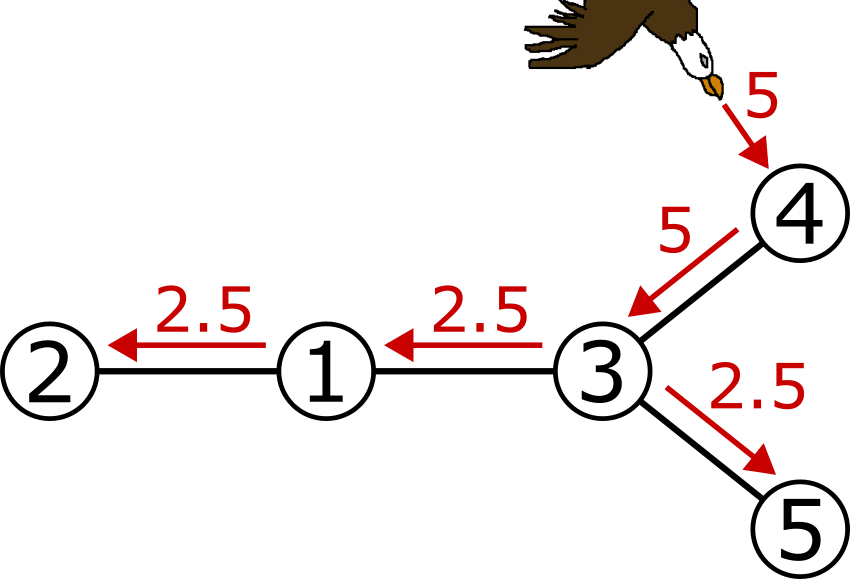
\includegraphics[width=0.8\textwidth]{a}
    \caption{Första örnen.}
    \label{fig:test1}
  \end{minipage}%
  \begin{minipage}{.5\textwidth}
    \centering
    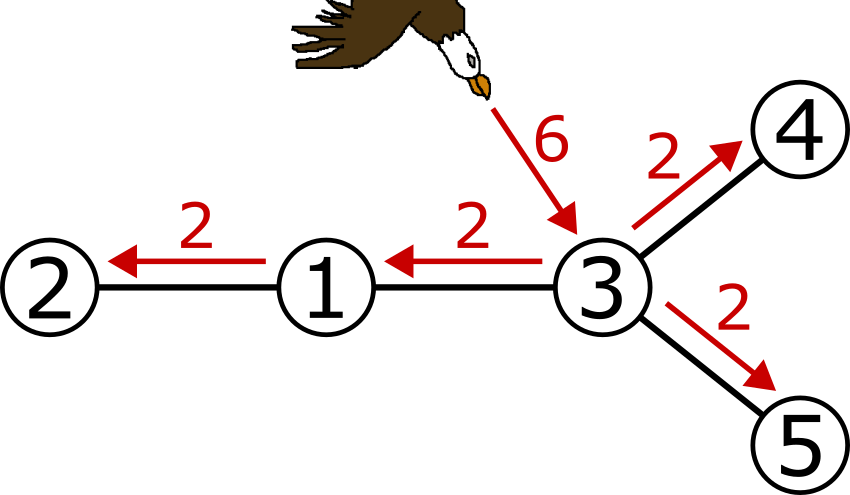
\includegraphics[width=0.8\textwidth]{b}
    \caption{Andra örnen.}
    \label{fig:test2}
  \end{minipage}
\end{figure}
      
      
Den första örnen kraschar i nod $4$ med fart $5$.
Från nod $4$ sprids skakningen endast till nod $3$ och från nod $3$ till både nod $1$ och $5$.
Från nod $5$ har skakningen ingenstans att ta vägen men från nod $1$ sprids den till nod $2$.

Den andra örnen kraschar i nod $3$ med fart $6$.
Från nod $3$ sprids skakningen till nod $1$, $4$ och $5$.
Skakningarna i nod $4$ och $5$ har ingenstans att ta vägen men skakningen i nod $1$ sprids till nod $2$.

För att få svaren ska varje nods skakningar adderas, exempelvis blir svaret $2.5+2=4.5$ i nod $1$ och $5+6=11$ i nod $3$.
